\documentclass[12pt]{amsart}
\bibliographystyle{amsalpha}
\usepackage{mathpazo,amssymb,amscd,epsfig,latexsym,graphicx,eucal}

\setlength\textheight{8in} 
\setlength\textwidth{6in}
\setlength\oddsidemargin{0.2in} 
\setlength\evensidemargin{0.2in}

\newcommand{\ds}{\displaystyle}
\newcommand{\diam}{\operatorname{diam}}
\newcommand{\area}{\operatorname{area}}
\newcommand{\dist}{\operatorname{dist}}
\newcommand{\ord}{\operatorname{ord}}
\newcommand{\myint}{\operatorname{int}}
\newcommand{\Aut}{\operatorname{Aut}}
\newcommand{\wtl}{\widetilde}
\newcommand{\wht}{\widehat}
\newcommand{\ve}{\varepsilon}
\newcommand{\es}{\emptyset}
\newcommand{\sm}{\smallsetminus}
\newcommand{\bd}{\partial}
\newcommand{\Chat}{\widehat{\Bbb C}}
\newcommand{\Real}{\operatorname{Re}}
\newcommand{\Image}{\operatorname{Im}}
\newcommand{\ov}{\overline}
\newcommand{\io}{\iota}
\newcommand{\con}{\operatorname{const.}}
\newcommand{\res}{\operatorname{res}}
\newcommand{\OO}{{\mathcal O}}
\newcommand{\MM}{{\mathcal M}}
\newcommand{\CC}{{\mathbb C}}
\newcommand{\PP}{{\mathbb P}}
\newcommand{\RR}{{\mathbb R}}
\newcommand{\HH}{{\mathbb H}}
\newcommand{\TT}{{\mathbb T}}
\newcommand{\II}{{\mathbb I}}
\newcommand{\ZZ}{{\mathbb Z}}
\newcommand{\NN}{{\mathbb N}}
\newcommand{\DD}{{\mathbb D}}
\newcommand{\QQ}{{\mathbb Q}}
\newcommand{\vs}{\vspace{2mm}}
\newcommand{\vr}{\varrho}
\newcommand{\iso}{\stackrel{\cong}{\longrightarrow}}
\newcommand{\Cbar}{\overline{\mathbb  C}}
\newcommand{\Cstar}{{\mathbb  C}^*}
\newcommand{\Dstar}{{\mathbb  D}^*}
\newcommand{\Sen}{{\mathbb  S}^1}

\font\bit=cmssi12 at 12truept \font\sbit=cmssi12 at 10truept

%Discourage hyphenation:
\hyphenpenalty=5000 \tolerance=1000

\thispagestyle{empty}

\begin{document}
\begin{center}
{\bf \large Math 704 Problem Set 1} \vs \\
{\bf due Friday 2/7/2025} \vs \vs
\end{center}

\noindent
{\bf Problem 1.} Prove the following form of Cauchy's criterion for convergence of infinite products: $\prod_{n=1}^{\infty} a_n$ converges if and only if for every $\ve>0$ there is an integer $N$ such that $|\prod_{n=m}^k a_n -1|<\ve$ whenever $k \geq m \geq N$. (Hint: The ``only if'' part is discussed in Remark 8.3. For the ``if'' part use logarithms.) \vs 

\noindent
{\bf Problem 2.} Consider a sequence $\{ C_n \}_{n=1}^{\infty}$ of concentric circles of increasing radii. For each $n$, the circle $C_n$ is inscribed in a regular $(n+2)$-gon and circumscribes a regular $(n+1)$-gon. Determine whether or not the radius of $C_n$ tends to infinity as $n \to \infty$. (Hint: First verify the relation $r_{n+1}=r_n \sec \theta_n$, where $r_n$ is the radius of $C_n$ and $\theta_n = \pi/(n+2)$.) \vs

%%%%%%%%%%%%%%%%%%%%%%%%%%%%%%%%%%%%%%%%%%%
\begin{figure}[h]
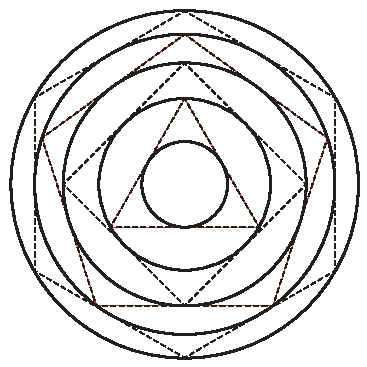
\epsfig{file=polygons.pdf, width=5cm}
\end{figure} 
%%%%%%%%%%%%%%%%%%%%%%%%%%%%%%%%%%%%%%%%%%%

\noindent
{\bf Problem 3.} Let $f(z)=\prod_{n=0}^{\infty} (1+z^{2^n})$. \vs
\begin{enumerate}
\item[(i)]
Show that the infinite product converges compactly in $\DD$, so $f \in \OO(\DD)$. \vs
\item[(ii)]
Let $p_k(z)=\prod_{n=0}^k (1+z^{2^n})$. Show that $p_k(z)=(1+z)p_{k-1}(z^2)$, and justify the functional equation $f(z)=(1+z)f(z^2)$. \vs
\item[(iii)]
Conclude that $f(z)=1/(1-z)$. \vs
\item[(iv)]
What does the resulting identity
$$
(1+z)(1+z^2)(1+z^4)(1+z^8) \cdots = 1+z+z^2+z^3+\cdots 
$$
for $|z|<1$ tell you about the binary expansion of integers? \vs
\end{enumerate}

\noindent
{\bf Problem 4.} In this exercise you will prove {\it Euler's product formula} (1734):
$$
\sin z = z \ \prod_{n=1}^{\infty} \left( 1-\frac{z^2}{\pi^2 n^2} \right) \qquad z \in \CC.
$$
The proof is deliberately divided into small steps for more clarity. \vs
\begin{enumerate}
\item[(i)]
Show that the above infinite product converges compactly in $\CC$ to an entire function $f$ with a simple zero at $\pi n$ for every $n \in \ZZ$, and with no other zeros. \vs
\item[(ii)]
Show that $\sin z / f(z)$ has removable singularities at every $\pi n$, so it is an entire function with no zeros. Conclude that for some entire function $g$,
$$
\sin z = e^{g(z)}\ z\ \prod_{n=1}^{\infty} \left( 1-\frac{z^2}{\pi^2 n^2} \right).
$$
\item[(iii)]
Use logarithmic differentiation to show that
$$
\cot z = g'(z)+\frac{1}{z}+\sum_{n=1}^{\infty} \left( \frac{1}{z-\pi n}+ \frac{1}{z+\pi n} \right),
$$
and hence
$$
g''(z)=- \frac{1}{\sin^2 z}+\sum_{n=-\infty}^{\infty} \frac{1} {(z-\pi n)^2}.
$$
Show that the right hand side is invariant under the translation $z \mapsto z+\pi$, that is, $g''(z+\pi)=g''(z)$. Prove the estimate
$$
|g''(z)| \leq \frac{1}{\sinh^2 y} + 2 \ \sum_{n=0}^{\infty} \frac{1}{(\pi^2 n^2+y^2)} \qquad (z=x+iy)
$$
provided that $0 \leq x \leq \pi$. Use Liouville's theorem to conclude that $g''=0$ and hence $g'$ is constant. \vs
\item[(iv)]
The right hand side of the first identity in (iii) is an odd function. Show that this gives $g' = 0$, so $g$ is constant. Use
(ii) to conclude that $g = 0$. \vs
\end{enumerate}

\noindent
{\bf Problem 5.} Use the results of the previous problem to calculate 
$$
\prod_{n=1}^{\infty} \left( 1+\frac{1}{n^2} \right) \quad \text{and} \quad \sum_{n=1}^{\infty} \frac{1}{n^2}. \vs
$$

\noindent
{\bf Problem 6.} Use the identity $\sin (2x) = 2 \sin x \, \cos x$ to show that
$$
\prod_{n=2}^{\infty} \cos \left( \frac{\pi}{2^n} \right) = \frac{2}{\pi}.
$$
Combine with the identity $\cos(2x)=2\cos^2 x -1$ to deduce {\it Veita's formula} (1579):
$$
\frac{2}{\pi} = \frac{\sqrt 2}{2} \cdot \frac{\sqrt{2+\sqrt{2}}}{2} \cdot \frac{\sqrt{2+\sqrt{2+\sqrt{2}}}}{2} \cdots \vs
$$


\end{document}
